\documentclass[compress]{beamer}
\usepackage{ifthen,verbatim}

\title{Very Early Alignment Plans}
\author{Jim Pivarski, Alexei Safonov, K\'aroly Banicz$^*$}
\institute{Texas A\&M University, $^*$FermiLab}
\date{5 Feb, 2008}

\newcommand{\isnote}{}
\xdefinecolor{lightyellow}{rgb}{1.,1.,0.25}
\xdefinecolor{darkblue}{rgb}{0.1,0.1,0.7}

%% Uncomment this to get annotations
%% \def\notes{\addtocounter{page}{-1}
%%            \renewcommand{\isnote}{*}
%% 	   \beamertemplateshadingbackground{lightyellow}{white}
%%            \begin{frame}
%%            \frametitle{Notes for the previous page (page \insertpagenumber)}
%%            \itemize}
%% \def\endnotes{\enditemize
%% 	      \end{frame}
%%               \beamertemplateshadingbackground{white}{white}
%%               \renewcommand{\isnote}{}}

%% Uncomment this to not get annotations
\def\notes{\comment}
\def\endnotes{\endcomment}

\setbeamertemplate{navigation symbols}{}
\setbeamertemplate{headline}{\includegraphics[height=1 cm]{../cmslogo} \hspace{0.1 cm} \includegraphics[height=1 cm]{../tamulogo} \hfill
\begin{minipage}{5.5 cm}
\vspace{-0.75 cm} \small
\begin{center}
\ifthenelse{\equal{\insertpagenumber}{1}}{}{\textcolor{blue}{\insertsection}}
\end{center}
\end{minipage} \hfill
\begin{minipage}{4.5 cm}
\vspace{-0.75 cm} \small
\begin{flushright}
\ifthenelse{\equal{\insertpagenumber}{1}}{}{Jim Pivarski \hspace{0.5 cm} \insertpagenumber\isnote/\pageref{numpages}}
\end{flushright}
\end{minipage}\mbox{\hspace{0.2 cm}}}

\begin{document}
\frame{\titlepage}

%% \begin{notes}
%% \item This is the annotated version of my talk.
%% \item If you want the version that I am presenting, download the one
%% labeled ``slides'' on Indico (or just ignore these yellow pages).
%% \item The annotated version is provided for extra detail and a written
%% record of comments that I intend to make orally.
%% \item Yellow notes refer to the content on the {\it previous} page.
%% \item All other slides are identical for the two versions.
%% \end{notes}

\begin{frame}
\frametitle{Overview}
\vspace{-1.2 cm}
\begin{center}
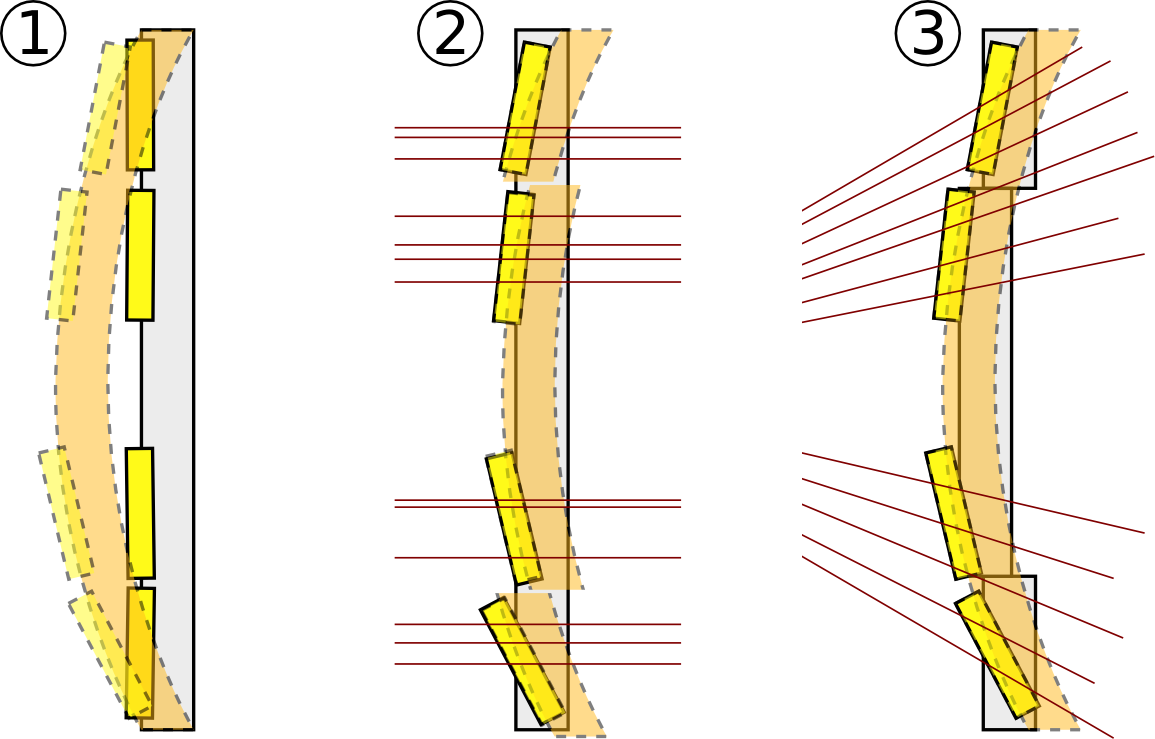
\includegraphics[width=0.7\linewidth]{plan.png}
\end{center}
\begin{enumerate}
\item Chambers start misaligned relative to ideal positions on each
ring, partly due to disk bending, and disk is misaligned relative to
its ideal position
\item Align chambers relative to one another on each ring using
beam-halo tracks in the CSC overlap regions
\item Align rings as large rigid bodies relative to the tracker using
first collision events
\end{enumerate}
\end{frame}

\begin{frame}
\frametitle{Beam-halo goals}
\textcolor{darkblue}{Goal 1:} Relative alignment of all chambers
within each ring using beam-halo tracks through CSC overlap regions
\begin{itemize}
\item Global position of whole ring (relative to other rings) is unconstrained by this procedure
\item Only adjacent chambers in the same ring overlap
\item Can't do ME1/3: no overlap regions and far from beam
\item Before collisions, wide-open trigger to collect all beam-halo
\item After collisions, use specialized beam-halo trigger
\end{itemize}

\textcolor{darkblue}{Goal 2:} Relative alignment of all CSC layers
within each ring using the same tracks
\begin{itemize}
\item Same technique, but let individual layers float
\item Since chamber alignment is applied first, ``chamber positions''
will be the average of the layer positions (the real detectors)
\end{itemize}
\end{frame}

\begin{frame}
\frametitle{Beam-halo procedure}
\begin{itemize}
\item Even-numbered chambers always overlap odd-numbered
\item Fit each beam-halo track to only one chamber, align partner
\begin{itemize}
\item APEs = 0 for half of disk of interest, APEs = $\infty$ elsewhere
\end{itemize}
\item Alternate between fitting to evens, aligning odds (1\&2) and
fitting to odds, aligning evens (3\&4)
\end{itemize}

\begin{center}
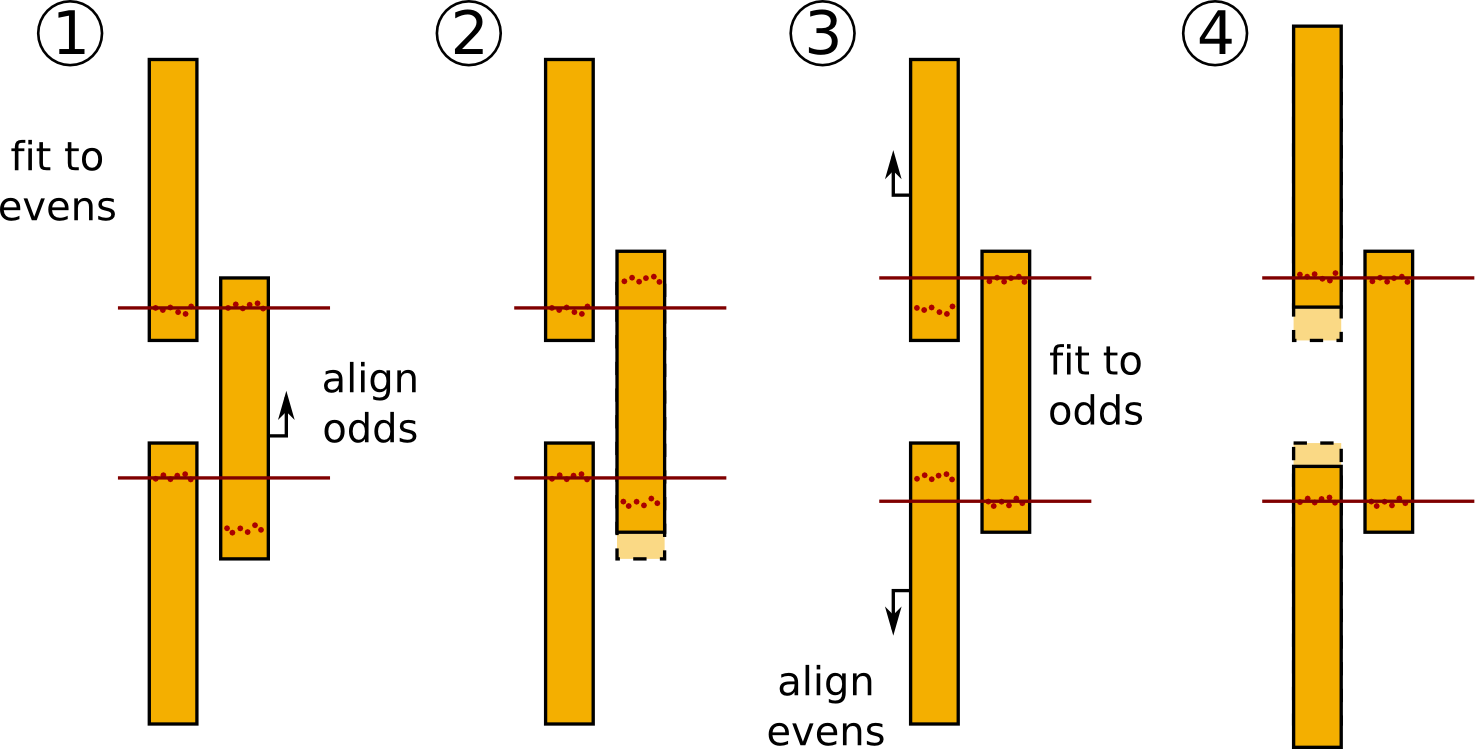
\includegraphics[width=0.75\linewidth]{beamhalo.png}
\end{center}
\end{frame}

\begin{frame}
\frametitle{Ring/Disk alignment procedure}
\begin{columns}
\column{0.6\linewidth}
\begin{itemize}
\item Disks (CSCStations) can be aligned as rigid bodies with only several hundred tracks
\item Beam-halo alignment procedure internally aligns rings, not disks

\vspace{0.1 cm}
Disks: \hfill ME1, ME2, ME3, ME4

Rings: \hfill 1/1a, 1/1b, 1/2, 1/3, 2/1, \\ \mbox{ } \hfill 2/2, 3/1, 3/2, 4/1\textcolor{white}{,}

\item Software issue:
\begin{itemize}
\item CSCRing not implemented in hierarchy (between CSCStation and CSCChamber)
\item Unrealistic to implement before CMSSW\_2\_0\_0
\item Work in checked-out code?
\end{itemize}
\end{itemize}

\column{0.4\linewidth}
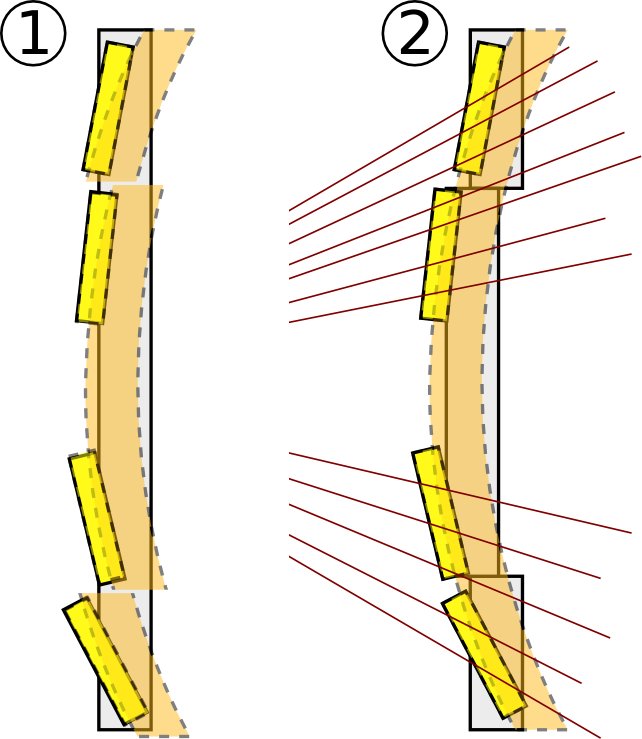
\includegraphics[width=\linewidth]{plan2.png}
\end{columns}
\end{frame}

\begin{frame}
\frametitle{Opportunities to compare with hardware alignment (1)}
\begin{itemize}
\item We can use ``survey constraints'' mechanism to constrain at
different levels of hierarchy, e.g.\ disk only
\item Technique to \underline{\it compare} beam-halo and hardware by applying constraints:
\begin{enumerate}
\item In beam-halo alignment, constrain disks' $x$, $y$, $z$, $\phi_z$ to hardware measurement
\item Compare beam-halo and hardware measurements of local $x$ positions of chambers (which is global $r\phi$)
\end{enumerate}
\item \textcolor{darkblue}{\#1} does not interfere with beam-halo
procedure, since that procedure doesn't measure disk positions anyway
\item Puts beam-halo chamber positions in the same coordinate
system as Straight Line Monitors: {\it comparison is meaningful}
\item Bonus: stabilizes beam-halo alignment
\end{itemize}
\end{frame}

\begin{frame}
\frametitle{Opportunities to compare with hardware alignment (2)}
\begin{itemize}\setlength{\itemsep}{0.25 cm}
\item One more comparison, starting from disk (hardware) and chamber (beam-halo) alignment
\begin{enumerate}
\setcounter{enumi}{2}
\item Align rings using standard technique: fitting tracks to tracker only (muon APEs = $\infty$)
\end{enumerate}
\item Fixing tracks to tracker makes track-based ring alignment independent of starting positions of muon disks
\item Track-based result minus hardware result is change in alignment parameters (small numbers)
\item Full 4-D test ($x$, $y$, $z$, $\phi_z$) of Transfer Lines, Link System, all the way from muon endcap to tracker
\item If there is a difference, we have ways to diagnose (residuals at
chamber level, inner ring vs.\ outer ring, etc.)
\end{itemize}

\label{numpages}
\end{frame}

\end{document}
